\documentclass[10pt,twocolumn]{article}
\usepackage[letterpaper,margin=0.75in,columnsep=0.25in]{geometry}
\usepackage[T1]{fontenc}
\usepackage{times}
\usepackage[hyphens]{url}
\usepackage[colorlinks=true,linkcolor=black,citecolor=blue!50!black,urlcolor=blue!50!black]{hyperref}
\usepackage{graphicx,booktabs,makecell,multirow,xcolor,pifont,microtype,amsmath,caption}
\usepackage[numbers,sort&compress]{natbib}
\newcommand{\NTwobrealcord}{0.59}
\newcommand{\NTwobrealfintabnet}{0.36}
\newcommand{\NTwobrealpubtabnet}{0.30}
\newcommand{\NTwobtest}{0.53}
\newcommand{\NTwobtestreceipt}{0.67}
\newcommand{\NTwobunseentabrecset}{0.31}
\newcommand{\NFourbrealcord}{0.79}
\newcommand{\NFourbrealfintabnet}{0.48}
\newcommand{\NFourbrealpubtabnet}{0.48}
\newcommand{\NFourbtest}{0.67}
\newcommand{\NFourbtestreceipt}{0.77}
\newcommand{\NFourbunseentabrecset}{0.38}
\newcommand{\NEightbhtmlrealcord}{0.44}
\newcommand{\NEightbhtmlrealfintabnet}{0.87}
\newcommand{\NEightbhtmlrealpubtabnet}{0.78}
\newcommand{\NEightbhtmltest}{0.47}
\newcommand{\NEightbhtmltestreceipt}{0.38}
\newcommand{\NEightbhtmlunseentabrecset}{0.58}
\newcommand{\NEightbsqlrealcord}{0.76}
\newcommand{\NEightbsqlrealfintabnet}{0.59}
\newcommand{\NEightbsqlrealpubtabnet}{0.52}
\newcommand{\NEightbsqltest}{0.75}
\newcommand{\NEightbsqltestreceipt}{0.87}
\newcommand{\NEightbsqlunseentabrecset}{0.45}
\newcommand{\NerrEightbhtmlcell}{79}
\newcommand{\NerrEightbhtmlcorrect}{28}
\newcommand{\NerrEightbhtmlkeyvalue}{1}
\newcommand{\NerrEightbhtmlno}{19}
\newcommand{\NerrEightbhtmlrow}{23}
\newcommand{\NerrEightbsqlcell}{69}
\newcommand{\NerrEightbsqlcorrect}{14}
\newcommand{\NerrEightbsqlkeyvalue}{2}
\newcommand{\NerrEightbsqlno}{27}
\newcommand{\NerrEightbsqlrow}{38}
\newcommand{\Nerrourscell}{76}
\newcommand{\Nerrourscorrect}{22}
\newcommand{\Nerrourskeyvalue}{2}
\newcommand{\Nerroursno}{21}
\newcommand{\Nerroursrow}{29}
\newcommand{\NfkTwob}{0.23}
\newcommand{\NfkFourb}{0.25}
\newcommand{\NfkEightbhtml}{0.00}
\newcommand{\NfkEightbsql}{0.75}
\newcommand{\Nfkours}{0.99}
\newcommand{\NkvfoneEightbhtml}{0.58}
\newcommand{\Nkvfoneours}{0.05}
\newcommand{\Nlvhtmla}{0.85}
\newcommand{\Nlvhtmlb}{0.84}
\newcommand{\Nlvhtmlc}{0.18}
\newcommand{\Nlvhtmld}{0.21}
\newcommand{\Nlvhtmle}{0.16}
\newcommand{\Nlvhtmlf}{0.57}
\newcommand{\Nlvoursa}{0.86}
\newcommand{\Nlvoursb}{0.90}
\newcommand{\Nlvoursc}{0.89}
\newcommand{\Nlvoursd}{0.95}
\newcommand{\Nlvourse}{0.90}
\newcommand{\Nlvoursf}{0.63}
\newcommand{\Nnkv}{2}
\newcommand{\NnokvfoneEightbhtml}{0.58}
\newcommand{\Nnokvfoneours}{0.53}
\newcommand{\Nntrainused}{36{,}589}
\newcommand{\Noursrealcord}{0.93}
\newcommand{\Noursrealfintabnet}{0.96}
\newcommand{\Noursrealpubtabnet}{0.81}
\newcommand{\Nourstest}{0.86}
\newcommand{\Nourstestreceipt}{1.00}
\newcommand{\Noursunseentabrecset}{0.52}
\newcommand{\Nprealcord}{0.000}
\newcommand{\Nprealfintabnet}{0.000}
\newcommand{\Nprealpubtabnet}{0.057}
\newcommand{\Nptest}{0.000}
\newcommand{\Nptestreceipt}{0.000}
\newcommand{\Npunseentabrecset}{0.000}
\newcommand{\NrepTwobexecraw}{0.78}
\newcommand{\NrepTwobexecrep}{0.87}
\newcommand{\NrepTwobfOneraw}{0.57}
\newcommand{\NrepTwobfOnerep}{0.61}
\newcommand{\NrepFourbexecraw}{0.97}
\newcommand{\NrepFourbexecrep}{0.99}
\newcommand{\NrepFourbfOneraw}{0.73}
\newcommand{\NrepFourbfOnerep}{0.73}
\newcommand{\NrepEightbsqlexecraw}{0.96}
\newcommand{\NrepEightbsqlexecrep}{1.00}
\newcommand{\NrepEightbsqlfOneraw}{0.77}
\newcommand{\NrepEightbsqlfOnerep}{0.78}
\newcommand{\Nrepoursexecraw}{0.96}
\newcommand{\Nrepoursexecrep}{0.99}
\newcommand{\NrepoursfOneraw}{0.90}
\newcommand{\NrepoursfOnerep}{0.91}
\newcommand{\Ntokhtml}{405}
\newcommand{\Ntokours}{195}
\newcommand{\Nvonerealcord}{0.49}
\newcommand{\Nvonerealfintabnet}{0.45}
\newcommand{\Nvonerealpubtabnet}{0.43}
\newcommand{\Nvonetest}{0.85}
\newcommand{\Nvonetestreceipt}{0.32}
\newcommand{\Nvoneunseentabrecset}{0.44}


\newcommand{\cmark}{\ding{51}}
\newcommand{\xmark}{\textcolor{black!35}{\ding{55}}}
\newcommand{\pmark}{$\circ$}
\newcommand{\sys}{\textsc{pix2db}}
\captionsetup{font=small,labelfont=bf}

\title{\sys: Reconstructing Executable Relational Databases\\from Document Images with a 2B Vision-Language Model}
\author{Musa Peker\\{\small Ozveri R\&D Center, Ozdilek Home Textile Industry and Trade Inc., Bursa, T\"urkiye}\\{\small\texttt{msapeker@gmail.com}}}
\date{}

\begin{document}
\maketitle

\begin{abstract}
Tables trapped in screenshots, scans, receipts and charts are usually extracted as markup that keeps the layout
but not the relational meaning: merged cells stay merged, an invoice header and its line items stay unrelated,
and ``\$1,250.00'' stays a string. We study \emph{image-to-database reconstruction}: given one image, produce a
SQLite dump whose schema, column types, keys and rows load and can be queried as they are. Training data with
exact gold databases is obtained in two ways: by rendering samples of the Spider databases at six layout levels,
and by converting PubTabNet, FinTabNet and CORD annotations under the same normalization rules. A 2B model
(Qwen3-VL-2B with LoRA) trained on \Nntrainused{} pairs and followed by a deterministic verify-and-repair layer
reaches \Nourstest{} table exact match and \Nfkours{} foreign-key recall on rendered tables from unseen databases,
against \NEightbsqltest{}/\NfkEightbsql{} for the 8B model of the same family prompted for SQL and
\NEightbhtmltest{}/\NfkEightbhtml{} for an 8B HTML-to-SQLite pipeline. On held-out real images it obtains cell F1
\Noursrealpubtabnet{} (PubTabNet) and \Noursrealfintabnet{} (FinTabNet) and recall \Noursrealcord{} on CORD receipt
photos. On TabRecSet, a source never seen in training, it is the best system that writes a database directly
(\Noursunseentabrecset{}) but trails the 8B HTML pipeline (\NEightbhtmlunseentabrecset{}), mostly in reading text
from photographs. A variant trained on synthetic data alone matches the synthetic score and fails on real
images, which locates the value of the real data. Code, model, data and all evaluation outputs are public.
\end{abstract}

% ------------------------------------------------------------------------------------------------
\section{Introduction}

A spreadsheet exported as a picture, a scanned statement, the photo of a receipt: in each case the data has a
relational structure that the image hides. Document understanding systems recover this structure as cell
grids~\citep{zhong2020pubtabnet,smock2022pubtables,nassar2022tableformer}, as HTML or Markdown produced by
OCR-free models~\citep{kim2022donut,lee2023pix2struct,blecher2023nougat,wei2024got,poznanski2025olmocr}, or as
linearized tables for charts~\citep{liu2023deplot}. These outputs describe how the table \emph{looks}. Turning
them into something a program can join, sum or filter still requires decisions that the markup leaves open:
which rows a merged cell belongs to, how a two-level header becomes a column name, whether ``(1,209)'' is a
negative number, and which of two tables on a page refers to the other.

We make these decisions part of the model's output. Given an image, \sys{} writes a SQLite dump
(\texttt{CREATE TABLE} with types, primary and foreign keys, followed by \texttt{INSERT} statements) that is
executed by an unmodified SQLite engine (Figure~\ref{fig:teaser}). The closest prior work,
OptiSQL~\citep{li2026optisql}, generates one SQL \emph{query} per question from a clean table image; we instead
reconstruct the database once, after which every query is ordinary SQL.

The task is not solved by prompting. In a pilot on 150 rendered images, Qwen3-VL-8B~\citep{bai2025qwen3vl} asked
for a SQL dump produced executable output 93\% of the time but a fully correct table only 61\% of the time, and
the same model asked for HTML that a 20-line script loads into SQLite reached 46\%, failing on exactly the
merged cells and forms that motivate the task. The errors were rarely misread characters. The models placed
merged values in one row, invented header tables, dropped foreign keys, or wrote \texttt{O'Brien} unescaped so
that one bad row voided an entire \texttt{INSERT}.

\begin{figure}[t]
\centering
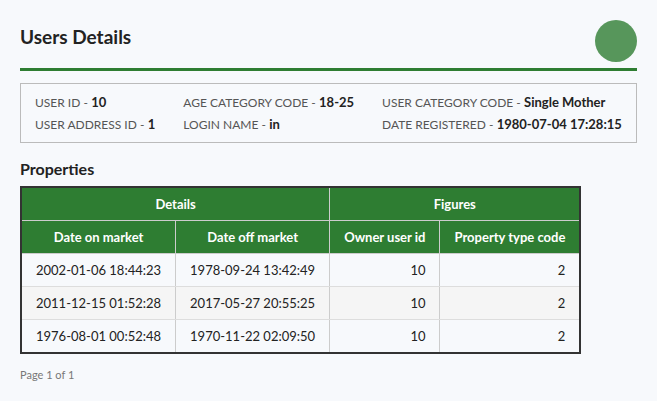
\includegraphics[width=0.62\linewidth]{figures/teaser_doc.png}\\[3pt]
\begin{minipage}{0.98\linewidth}
{\fontsize{6.1}{6.9}\selectfont
\begin{verbatim}
CREATE TABLE users (user_id INTEGER PRIMARY KEY,
  age_category_code TEXT, user_category_code TEXT,
  user_address_id INTEGER, login_name TEXT,
  date_registered TEXT);
CREATE TABLE properties (date_on_market TEXT,
  date_off_market TEXT, owner_user_id INTEGER,
  property_type_code INTEGER,
  FOREIGN KEY (owner_user_id) REFERENCES users(user_id));
INSERT INTO users VALUES
  (10, '18-25', 'Single Mother', 1, 'in', '1980-07-04 17:28:15');
INSERT INTO properties VALUES
  ('2002-01-06 18:44:23', '1978-09-24 13:42:49', 10, 2), ...
\end{verbatim}}
\end{minipage}
\caption{A rendered document from an unseen database and the dump written by \sys{} (abridged). The key--value
header becomes its own table, the merged \emph{Owner Id} cell is repeated in every item row, and the relation
between the two blocks is stated as a foreign key.}
\label{fig:teaser}
\end{figure}

\paragraph{Contributions.}
\begin{itemize}\setlength\itemsep{1pt}
\item A task definition for image-to-database reconstruction with explicit normalization conventions, and an
evaluation protocol that aligns predicted and gold databases without relying on table or column names
(\S\ref{sec:task}).
\item A data recipe that yields exact gold databases at scale: rendering samples of real relational databases at
controlled layout difficulty, and converting existing table and receipt annotations into the same conventions,
with every gold dump verified by execution (\S\ref{sec:data}).
\item \sys-2b, a 2B model with a deterministic verify-and-repair layer, which outperforms 4$\times$ larger models
of its family on five of six evaluation sets and recovers foreign keys almost perfectly (\S\ref{sec:results}).
\item An analysis of what transfers: synthetic layouts teach normalization but not reading, a modest converted real
set closes most of the real-image gap, and on a truly unseen source the remaining gap is reading accuracy rather
than structure (\S\ref{sec:results}--\ref{sec:discussion}).
\end{itemize}

% ------------------------------------------------------------------------------------------------
\section{Related work}
\label{sec:related}

\paragraph{Table structure recognition.} TSR predicts the cell grid of a cropped table, evaluated with the
tree-edit-distance score TEDS~\citep{zhong2020pubtabnet}. Large annotated corpora come from scientific
articles~\citep{zhong2020pubtabnet,smock2022pubtables,chi2019scitsr} and financial reports~\citep{zheng2021gte},
and photographed tables are covered by WTW~\citep{long2021wtw} and TabRecSet~\citep{yang2023tabrecset}.
TableFormer~\citep{nassar2022tableformer} and the PubTables-1M detector~\citep{smock2022pubtables} predict
structure and rely on PDF text or OCR for content. A grid is a faithful description of the layout, not of the data:
TEDS rewards reproducing a rowspan, whereas a database must resolve it.

\paragraph{OCR-free document models.} Donut~\citep{kim2022donut} and Pix2Struct~\citep{lee2023pix2struct}
showed that an image-to-sequence model can parse documents without an OCR stage; Nougat~\citep{blecher2023nougat},
GOT~\citep{wei2024got}, olmOCR~\citep{poznanski2025olmocr} and Docling~\citep{auer2024docling} convert pages to
Markdown, LaTeX or HTML. General VLMs such as Qwen3-VL~\citep{bai2025qwen3vl} read tables well enough to be our
strongest baselines. None of these targets a typed relational schema or relations between tables.

\paragraph{Charts.} DePlot~\citep{liu2023deplot}, MatCha~\citep{liu2023matcha} and UniChart~\citep{masry2023unichart}
translate plots into linearized tables, with ChartQA~\citep{masry2022chartqa} and PlotQA~\citep{methani2020plotqa}
as standard benchmarks. We treat a chart as one more layout whose target is a typed table.

\paragraph{Tables, images and SQL.} Text-to-SQL benchmarks~\citep{yu2018spider,li2023bird,lei2025spider2} assume
the database already exists. Visual table QA~\citep{zheng2024multimodal,singh2025mtabvqa,mathew2021docvqa} answers
questions over images, and recent analyses report that VLMs degrade sharply on noisy real-world
tables~\citep{singh2025lost}. OptiSQL~\citep{li2026optisql} renders Spider~2.0 tables and generates an executable
query from the image and a question; its gold database is never reconstructed. MTabVQA~\citep{singh2025mtabvqa}
renders Spider and BIRD tables for multi-table QA. Our use of Spider is similar in spirit, but the database itself
is the output. Rendering synthetic training data with free and exact labels follows a long line of work in
OCR~\citep{gupta2016synthtext}.

Table~\ref{tab:capabilities} summarizes the differences.

\begin{table}[t]
\centering\small
\setlength{\tabcolsep}{3pt}
\resizebox{\linewidth}{!}{%
\begin{tabular}{lcccccc}
\toprule
& \rotatebox{70}{typed schema} & \rotatebox{70}{multi-table + FK} & \rotatebox{70}{spans resolved} & \rotatebox{70}{charts} & \rotatebox{70}{photos, receipts} & \rotatebox{70}{executable DB} \\
\midrule
TSR models~\citep{nassar2022tableformer,smock2022pubtables} & \xmark & \xmark & \xmark & \xmark & \pmark & \xmark \\
Page-to-markup~\citep{blecher2023nougat,poznanski2025olmocr,auer2024docling} & \xmark & \xmark & \xmark & \xmark & \pmark & \xmark \\
Donut-style parsing~\citep{kim2022donut} & \pmark & \xmark & \xmark & \xmark & \cmark & \xmark \\
Chart-to-table~\citep{liu2023deplot,masry2023unichart} & \xmark & \xmark & -- & \cmark & \xmark & \xmark \\
OptiSQL~\citep{li2026optisql} & -- & \xmark & \xmark & \xmark & \xmark & \xmark \\
\sys{} (ours) & \cmark & \cmark & \cmark & \cmark & \cmark & \cmark \\
\bottomrule
\end{tabular}}
\caption{Capabilities as described in the respective papers. \pmark: partly, or for a subset of inputs.
Donut-style parsers emit task-specific JSON fields; OptiSQL emits a query against an existing database.}
\label{tab:capabilities}
\end{table}

% ------------------------------------------------------------------------------------------------
\section{Task and evaluation}
\label{sec:task}

\paragraph{Output.} For an image $I$ the system outputs a SQL text $D$; the prediction is the database obtained by
executing the \texttt{CREATE TABLE} and \texttt{INSERT} statements of $D$ in an empty SQLite instance (other
statements are ignored). The target follows fixed conventions: one row per record, with the value of a merged
cell repeated in every row it covers; multi-level headers joined into one snake\_case name; numbers stored without
thousand separators or currency signs, accounting negatives as negative numbers; dates in ISO form; empty cells
as \texttt{NULL}; derived totals rows not stored; one table per logical block, with a foreign key from line items
to their header; for charts, the category and one column per series. Table and column names are chosen by the
model and are not scored.

\paragraph{Alignment.} Cell values are normalized (Unicode NFKC, dash variants unified, numbers parsed after
removing separators and currency, common date formats mapped to ISO, strings case-folded); empty values are
ignored. For a gold table $G$ and a predicted table $P$, columns are aligned by a maximum-weight bipartite matching
whose weights are the multiset overlap of normalized column values, and rows by a second matching whose weights
count agreeing aligned cells~\citep{kuhn1955hungarian}. The resulting number of agreeing cells $a(G,P)$ is used to
match gold to predicted tables, again by maximum-weight assignment.

\paragraph{Metrics.} \emph{Cell precision, recall and F1} divide the total of $a$ over matched tables by the number
of non-empty predicted and gold cells. \emph{Table exact match} requires a matched table with the same number of
rows and columns and every gold cell recovered. \emph{FK recall} is the fraction of gold foreign keys whose child
and parent tables are matched to predicted tables connected by a declared foreign key. \emph{Type accuracy} counts
an aligned column as correct when its declared SQLite affinity and the stored values agree with the gold column
being numeric or textual. Two cases are relaxed: values of charts drawn without value labels match within
$\tau = 0.04\cdot\max|v|$, and receipts are scored by recall, because a correct database may legitimately contain
an extra table for totals or payment.

% ------------------------------------------------------------------------------------------------
\section{Data}
\label{sec:data}

\begin{figure*}[t]
\centering
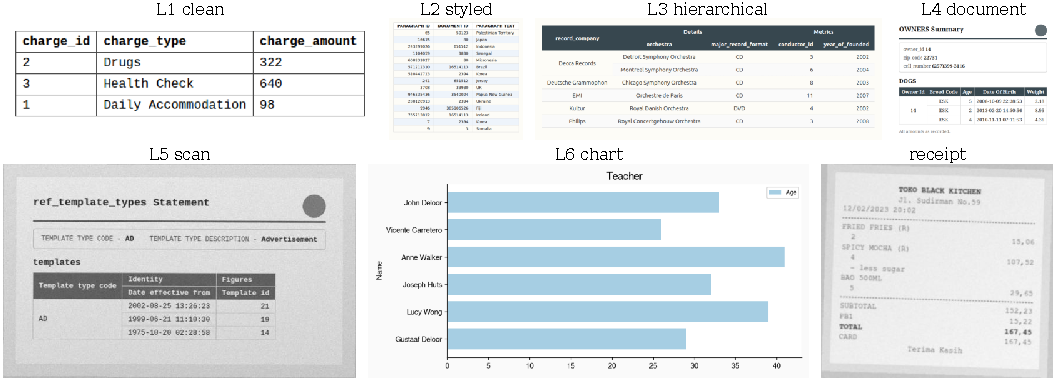
\includegraphics[width=\textwidth]{figures/renders.pdf}
\caption{One rendered example per synthetic level, all from the validation databases. Gold databases for these
images are exact by construction; for the receipt it is a single \texttt{items} table, and the subtotal, tax and
payment lines are not stored.}
\label{fig:renders}
\end{figure*}

\subsection{Rendering databases}
A \emph{scene} is a small database cut from one of the Spider~\citep{yu2018spider} SQLite files: a single table
with 3--25 sampled rows and 3--9 columns, two unrelated tables, or a parent row together with 3--15 child rows
that reference it through a declared foreign key. Columns with long or mostly empty values are dropped, numeric
strings and integer-valued floats are coerced to numbers, and composite primary keys are not declared.

Scenes are rendered with HTML/CSS in headless Chromium at six levels (Figure~\ref{fig:renders}).
\textbf{L1} draws a plain grid with raw column names. \textbf{L2} adds 17 font families, colored or zebra
styling, humanized headers in four case styles, thousand separators (never on identifiers or years), currency
prefixes on money-like columns and long-form dates. \textbf{L3} adds merged cells on a repeated grouping column,
two-level headers that group textual and numeric columns, transposed layouts for small tables and
occasional derived totals rows. \textbf{L4} renders a parent row as a key--value block above the child table. \textbf{L5} photographs L3 and
L4 pages with rotation up to $\pm2.5^\circ$, uneven lighting, sensor noise, blur, contrast change, optional
grayscale and JPEG quality 45--80. \textbf{L6} draws bar, horizontal bar, line and pie charts with one to three
series, printing value labels for 60\% of charts whose labels are exact. Synthetic receipts use monospaced
narrow layouts with three item-line formats, modifiers such as ``less sugar'', subtotal, tax and payment lines,
and are photographed 85\% of the time.

Two invariants keep the gold exact. Every displayed string maps back to the gold value without loss (formatting
adds separators or symbols, never rounds or truncates). And because rendering may reorder rows and columns, for
example to group merged cells, the gold scene is reordered the same way, so that the target dump reads in the
order of the image. Splits are made by database: the 146 Spider training databases feed training, the 20
development databases validation, and the 40 databases that appear only in Spider's test set our synthetic test.

\subsection{Converting real annotations}
PubTabNet~\citep{zhong2020pubtabnet} and FinTabNet~\citep{zheng2021gte} annotate table images with HTML. We expand
spans into a grid, flatten header rows into names, repeat body rowspans, convert numbers as above and map lone
dashes to \texttt{NULL}. FinTabNet tables carry no \texttt{thead}; the first row is used as header, and the second
as well when the first contains group colspans. Tables whose body contains colspans, typically section rows such as
``Assets'', have no unambiguous relational form and are rejected, as are tables with more than 30 rows or 10
columns. Of the streamed training tables, 72\% of PubTabNet and 69\% of FinTabNet pass. CORD~\citep{park2019cord}
receipts become an \texttt{items} table (name, quantity, price) built from the menu annotations.

\paragraph{Execution check.} Every gold dump, synthetic or converted, is executed and scored against itself; any
score below 1.0 is a bug in the data. The check found composite keys declared as primary keys, numbers stored as
text by Spider, identifiers that start with a digit or are SQL keywords (now quoted), empty strings in numeric
columns, and a header-deduplication collision in one converted table, which was removed.

\begin{table}[t]
\centering\small
\setlength{\tabcolsep}{4pt}
\begin{tabular}{lrrrrr}
\toprule
Split & images & tables/img & rows & cols & with FK \\
\midrule
train (synthetic) & 24,000 & 1.38 & 7.5 & 3.7 & 29\% \\
train (real) & 18,794 & 1.00 & 9.4 & 4.6 & 0\% \\
train (receipts) & 3,000 & 1.00 & 7.1 & 3.5 & 0\% \\
validation & 600 & 1.30 & 7.7 & 3.7 & 22\% \\
test (synthetic) & 900 & 1.32 & 7.0 & 3.4 & 24\% \\
test (receipts) & 150 & 1.00 & 6.8 & 3.5 & 0\% \\
PubTabNet (val) & 150 & 1.00 & 9.4 & 4.2 & 0\% \\
FinTabNet (val) & 150 & 1.00 & 8.5 & 4.6 & 0\% \\
CORD (test) & 60 & 1.00 & 3.5 & 3.0 & 0\% \\
TabRecSet (unseen) & 150 & 1.00 & 6.7 & 3.8 & 0\% \\
\bottomrule
\end{tabular}
\caption{Splits. Rows and columns are averages per table; ``with FK'' is the share of images whose gold contains a
foreign key. All splits are released.}
\label{tab:data}
\end{table}

\subsection{Evaluation sets}
Besides the synthetic test (150 images per level), we use held-out splits of the real sources: 150 PubTabNet and
150 FinTabNet validation tables and 60 CORD test receipts with at least two items, plus 150 synthetic receipts.
These images are unseen, but their style is familiar from training. To measure transfer we also build
\textbf{TabRecSet-150} from TabRecSet~\citep{yang2023tabrecset} (CC BY 4.0), which was never used for training:
English original images, one table per image, cropped by its cell polygons, with at least 60\% non-empty cells.
TabRecSet does not mark header rows, so the first grid row is used as header; 64\% of the inspected tables pass
the same conversion rules. Table~\ref{tab:data} lists all splits.

% ------------------------------------------------------------------------------------------------
\section{Model and repair layer}
\label{sec:model}

\paragraph{Model.} \sys-2b is Qwen3-VL-2B-Instruct~\citep{bai2025qwen3vl} with LoRA~\citep{hu2022lora} (rank 64,
$\alpha=128$, dropout 0.05) on all attention and MLP projections of the language model; the vision encoder is
frozen. Images are resized to at most 1.31\,MP (about 1{,}280 visual tokens). The loss covers only the answer,
a fenced SQL block. Training mixes 14k synthetic images (all six levels), 3k synthetic receipts, 10k PubTabNet,
8k FinTabNet and 795 CORD receipts seen twice: \Nntrainused{} examples, one epoch, effective batch 16, learning rate
$10^{-4}$ with cosine decay and 3\% warm-up, bf16, 2{,}287 steps in 5.9 hours on one A40. The adapter is merged
into the base weights for release. A per-device batch of 8 ran out of memory on long batches because of the full
vocabulary logits, so we used 4 with gradient accumulation of 4.

\paragraph{Verify and repair.} Model output passes through a deterministic layer before it is returned. Statements
are executed one at a time; a failing statement is retried after escaping apostrophes inside words, quoting or
rewriting identifiers that are SQL keywords or free text (\texttt{\# of sequences\textsuperscript{1}}
$\rightarrow$ \texttt{of\_sequences}), and, for \texttt{INSERT}s, inserting row by row with bare composite values
(\texttt{9 (8)}, \texttt{85.0 ± 10.8}) quoted as text and missing trailing cells padded with \texttt{NULL}. A primary
key that rejects duplicate values is dropped rather than the rows. Truncated output keeps its complete tuples.
Remaining problems are reported, not hidden: empty tables, values that contradict their declared type, duplicate
rows and foreign keys without a parent. Statements that execute are left as they are, except that a primary key
is dropped when later rows violate it.

% ------------------------------------------------------------------------------------------------
\section{Experiments}
\label{sec:results}

\paragraph{Baselines.} We compare with Qwen3-VL-2B, 4B and 8B-Instruct given the same instruction as \sys{}
(Appendix~\ref{app:prompt}), and with a two-stage pipeline in which Qwen3-VL-8B outputs HTML tables that keep
row and column spans, and a script loads them with \texttt{pandas.read\_html} (which expands spans) into SQLite.
All SQL outputs, ours and the baselines', go through the same repair layer. Decoding is greedy with at most 3{,}072
new tokens, served by vLLM~\citep{kwon2023vllm}. 95\% confidence intervals come from 2{,}000 bootstrap resamples of
evaluation items, and $p$-values from a one-sided paired bootstrap against the strongest competitor on each set.

\begin{table*}[t]
\centering\small
\setlength{\tabcolsep}{4.5pt}
\begin{tabular}{lccccccc}
\toprule
System & \makecell{Synthetic\\[-1pt]\scriptsize exact} & \makecell{PubTabNet\\[-1pt]\scriptsize f1} & \makecell{FinTabNet\\[-1pt]\scriptsize f1} & \makecell{CORD\\[-1pt]\scriptsize recall} & \makecell{Synth. receipts\\[-1pt]\scriptsize recall} & \makecell{TabRecSet\\[-1pt]\scriptsize f1} & \makecell{FK\\[-1pt]\scriptsize recall} \\
\midrule
pix2db-2b (ours) & \textbf{0.86}\,{\tiny[0.83,0.88]} & \textbf{0.81}\,{\tiny[0.77,0.84]} & \textbf{0.96}\,{\tiny[0.95,0.98]} & \textbf{0.93}\,{\tiny[0.89,0.96]} & \textbf{1.00}\,{\tiny[1.00,1.00]} & 0.52\,{\tiny[0.47,0.57]} & \textbf{0.99} \\
\midrule
Qwen3-VL-8B $\to$ SQL & 0.75\,{\tiny[0.73,0.78]} & 0.52\,{\tiny[0.47,0.57]} & 0.59\,{\tiny[0.54,0.64]} & 0.76\,{\tiny[0.69,0.83]} & 0.87\,{\tiny[0.84,0.90]} & 0.45\,{\tiny[0.40,0.50]} & 0.75 \\
Qwen3-VL-8B $\to$ HTML $\to$ SQLite & 0.47\,{\tiny[0.44,0.50]} & 0.78\,{\tiny[0.75,0.82]} & 0.87\,{\tiny[0.84,0.89]} & 0.44\,{\tiny[0.36,0.52]} & 0.38\,{\tiny[0.34,0.42]} & \textbf{0.58}\,{\tiny[0.53,0.63]} & 0.00 \\
Qwen3-VL-4B $\to$ SQL & 0.67\,{\tiny[0.63,0.69]} & 0.48\,{\tiny[0.42,0.53]} & 0.48\,{\tiny[0.42,0.54]} & 0.79\,{\tiny[0.72,0.85]} & 0.77\,{\tiny[0.73,0.81]} & 0.38\,{\tiny[0.33,0.44]} & 0.25 \\
Qwen3-VL-2B $\to$ SQL (base) & 0.53\,{\tiny[0.50,0.56]} & 0.30\,{\tiny[0.25,0.36]} & 0.36\,{\tiny[0.31,0.41]} & 0.59\,{\tiny[0.49,0.68]} & 0.67\,{\tiny[0.62,0.72]} & 0.31\,{\tiny[0.26,0.36]} & 0.23 \\
\bottomrule
\end{tabular}
\caption{Main results with 95\% bootstrap intervals. Synthetic: table exact match on 900 images from unseen
databases; PubTabNet, FinTabNet, TabRecSet: cell F1; CORD and synthetic receipts: cell recall; FK recall on the
synthetic test images that contain a foreign key. Against the best competitor on each set, \sys{} is ahead with
$p<0.001$ on synthetic, FinTabNet, CORD and synthetic receipts and with $p=\Nprealpubtabnet$ on PubTabNet; on
TabRecSet the 8B HTML pipeline is ahead with $p<0.001$.}
\label{tab:main}
\end{table*}

\subsection{Main results}
Table~\ref{tab:main} gives the overall picture. Fine-tuning moves the 2B model from the bottom of the table to the
top on every set except TabRecSet. On the synthetic test it gains 33 points of exact match over its own base model
and 11 over the 8B model; on FinTabNet and CORD the margins over the strongest competitor are 9 and 14 points.
PubTabNet is the closest case: the HTML pipeline, which is well suited to flat scientific tables, is 3 points
behind and the difference is not significant at the 5\% level. Foreign keys separate the systems most clearly.
\sys{} declares \Nfkours{} of the gold relations, the 8B model prompted for SQL \NfkEightbsql{}, the smaller models
a quarter, and the HTML pipeline none, because nothing in HTML expresses a relation between two tables.

\begin{figure*}[t]
\centering
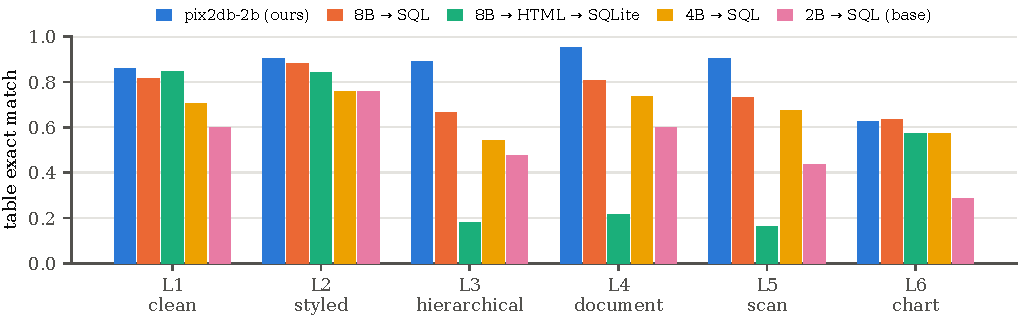
\includegraphics[width=0.94\textwidth]{figures/levels.pdf}
\caption{Table exact match per synthetic level (150 images each). The HTML pipeline is competitive on flat tables
and loses most of its accuracy once merged cells, forms or scanning are involved.}
\label{fig:levels}
\end{figure*}

\subsection{Where layout matters}
Figure~\ref{fig:levels} breaks the synthetic test down by level. On flat tables (L1, L2) every system is within a
few points of the others, and the HTML pipeline reaches \Nlvhtmla{} and \Nlvhtmlb{}. With merged cells, key--value
headers and photographed pages it falls to \Nlvhtmlc{}, \Nlvhtmld{} and \Nlvhtmle{}, whereas \sys{} stays at
\Nlvoursc{}, \Nlvoursd{} and \Nlvourse{}. The HTML stage itself is mostly right; the failure is in the
conversion, which has no notion that a rowspan is a grouping key or that a form above a table is a separate
record. Charts are the exception to the pattern: apart from the untuned 2B model, all systems lie between 0.57
and 0.63 exact match, and \sys{} (\Nlvoursf{}) is not better than the 8B model. Charts without value labels are
harder (0.52 exact against 0.69 with labels), but labeled charts still fail in almost a third of cases, so the
difficulty lies as much in assigning marks to categories and series as in estimating values.

\subsection{What the real data contributes}
We trained a first version, otherwise identical, on 24k synthetic images only. Figure~\ref{fig:ablation_data} shows
that it reaches the same synthetic accuracy (\Nvonetest{} vs.\ \Nourstest{}) and transfers poorly: cell F1
\Nvonerealpubtabnet{} on PubTabNet, \Nvonerealfintabnet{} on FinTabNet, recall \Nvonerealcord{} on CORD. Its
failures on PubTabNet were rarely layout errors. In 82 of 150 outputs the SQL did not execute at all (28 after
repair), mostly because composite values such as \texttt{9 (8)} or \texttt{85.0 ± 10.8} were written as bare numbers, a format
that never occurs in Spider, and in others the model looped on a \texttt{CREATE TABLE} it could not finish. Adding
18.8k converted real tables and receipts fixes this without costing synthetic accuracy and lifts TabRecSet from
\Nvoneunseentabrecset{} to \Noursunseentabrecset{}. The synthetic data teaches the conventions; the real data
teaches what real cell contents look like.

\begin{figure}[t]
\centering
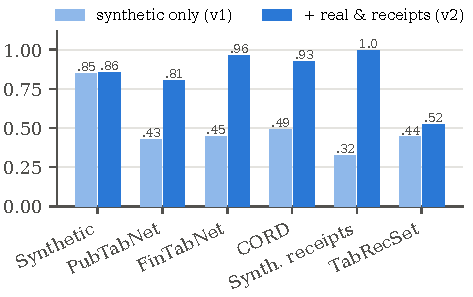
\includegraphics[width=\linewidth]{figures/ablation_data.pdf}
\caption{Same model and recipe, trained on synthetic data only (v1) or with the converted real tables and
receipts added (v2). Metrics as in Table~\ref{tab:main}.}
\label{fig:ablation_data}
\end{figure}

\subsection{Effect of the repair layer}
Figure~\ref{fig:ablation_repair} pools all six sets. The layer raises the share of outputs that execute from
\Nrepoursexecraw{} to \Nrepoursexecrep{} for \sys{} and from \NrepTwobexecraw{} to \NrepTwobexecrep{} for the
untuned 2B model, but it moves pooled cell F1 by at most four points. Its value lies in the tail: on TabRecSet, where
\sys{} is out of distribution, execution rises from 0.91 to 0.99, and on PubTabNet F1 improves by 3 points
(Appendix, Table~\ref{tab:repair}). Repair is no substitute for training. Applied to the base model it leaves
F1 at \NrepTwobfOnerep{}, far below the fine-tuned model without repair (\NrepoursfOneraw{}).

\begin{figure}[t]
\centering
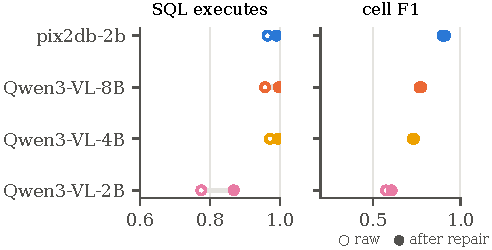
\includegraphics[width=0.93\linewidth]{figures/ablation_repair.pdf}
\caption{Share of executable outputs and cell F1 before and after the repair layer, pooled over all evaluation
sets.}
\label{fig:ablation_repair}
\end{figure}

\subsection{Unseen source: TabRecSet}
TabRecSet-150 is the only set on which \sys{} loses (\Noursunseentabrecset{} vs.\ \NEightbhtmlunseentabrecset{}).
We sorted each prediction into one category (Figure~\ref{fig:errors}): F1 of at least 0.9; usable output with the
right number of rows but wrong cell contents; a wrong number of rows; a two-column key--value table; or no usable
output. Key--value layouts, where our first-row-as-header gold is questionable, account for only \Nnkv{} tables
and do not explain the gap. The largest bucket for all systems is cell content
(\Nerrourscell{} for \sys{}, \NerrEightbhtmlcell{} for the HTML pipeline): the rows are found but text in
photographed, skewed or low-resolution tables is misread. \sys{} also segments rows wrongly more often
(\Nerroursrow{} vs.\ \NerrEightbhtmlrow{}). The 8B model reads these images better than the 2B model it is compared
with, and the HTML route spends no capacity on normalization. On this source the bottleneck is reading, which
points to a larger base model as the next step rather than more synthetic layouts.

\begin{figure}[t]
\centering
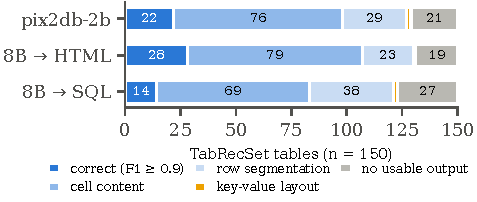
\includegraphics[width=\linewidth]{figures/errors_tabrecset.pdf}
\caption{Outcome categories on TabRecSet-150, a source never used in training.}
\label{fig:errors}
\end{figure}

\subsection{Types and cost}
Table~\ref{tab:types} adds column types and output size on the synthetic test. Stored types are almost always
right for every SQL system; the HTML pipeline gets 0.89 because pandas infers types from the formatted strings, so
``\$1,250'' stays text. \sys{} writes the shortest outputs (\Ntokours{} tokens on average, against \Ntokhtml{} for
HTML), which together with its size makes it the fastest system: 0.09\,s per image amortized over a vLLM batch on
one A40. Training and every evaluation in this paper used about 12 A40 GPU-hours.

\begin{table}[t]
\centering\small
\setlength{\tabcolsep}{3pt}
\begin{tabular}{lcccc}
\toprule
System & types & exec & tokens & s/img \\
\midrule
pix2db-2b (ours) & 0.99 & 0.96 & 195 & 0.09 \\
8B $\to$ SQL & 0.98 & 0.95 & 265 & 0.29 \\
8B $\to$ HTML $\to$ SQLite & 0.89 & -- & 405 & 0.34 \\
4B $\to$ SQL & 0.98 & 0.99 & 207 & 0.18 \\
2B $\to$ SQL (base) & 0.98 & 0.83 & 274 & 0.13 \\
\bottomrule
\end{tabular}
\caption{Synthetic test. Type accuracy over aligned columns (after repair), share of raw outputs that execute,
mean output tokens and amortized seconds per image with vLLM on one A40.}
\label{tab:types}
\end{table}

% ------------------------------------------------------------------------------------------------
\section{Discussion}
\label{sec:discussion}

\paragraph{Conventions are cheap to learn, reading is not.} The decisions that turn a layout into a database are
few and regular, and general VLMs know them but apply them inconsistently: the 8B model declares three quarters of
the foreign keys and merges cells correctly about two times in three. A small model trained on a few tens of
thousands of exact examples applies them almost every time. Reading text is different. The synthetic-only model
read rendered text perfectly and real text poorly, and on TabRecSet a larger general model still reads better
than our fine-tuned small one. We expect the recipe to carry over to a 4B or 8B base with little change, and the
TabRecSet gap to shrink accordingly.

\paragraph{The HTML route is a strong baseline for flat tables.} When a table has one header row and no merged
cells, ``copy the grid, let a script load it'' is hard to beat, and our PubTabNet result is statistically tied
with it. Its weaknesses are structural: it cannot express relations, it inherits pandas' type inference, and it
has no answer for rowspans that encode grouping. Systems that output markup should be evaluated with these cases
in view, which TEDS-style metrics do not reward.

\paragraph{Rendering from databases.} Starting from a database and producing the image inverts the usual
annotation effort: labels are exact, difficulty is a parameter, and the same scene can be shown with and without
merged cells or scanning. The cost is a narrow distribution of typography and cell contents, which the real-data
ablation makes visible. Converting existing annotations was the cheapest way to widen it; the converter is about
150 lines of code and rejects roughly 30\% of the tables it sees.

\paragraph{Validity of the evaluation.} The metric ignores names, so a schema with unhelpful column names scores
as well as a good one; naming quality is not measured. The real held-out sets share sources with training data
and therefore overstate performance on unfamiliar documents, which is why we report TabRecSet separately.
TabRecSet's missing header annotation forces a header assumption that is wrong for some tables, although the error
analysis shows it affects few. All numbers come from a single training run; the intervals reflect sampling of test
items, not training variance.

\paragraph{Limitations.} Handwriting, multi-page tables and tables longer than 30 rows are outside the training
distribution. Tables whose body contains section rows were excluded from both training and evaluation, so we do
not know how the model handles them. Charts without value labels are read approximately. All data is English.

\paragraph{Broader impact.} Receipts and invoices may contain personal data; the released data uses public
datasets whose images were collected and anonymized by their authors. Extraction errors are likely to look
plausible, so the warnings reported by the repair layer should be shown to users rather than discarded.

% ------------------------------------------------------------------------------------------------
\section{Conclusion}
Image-to-database reconstruction asks for decisions that markup leaves open, and a 2B model trained on exact
gold databases makes them reliably: merged cells become rows, forms become related tables, and the result runs
in SQLite. Rendered databases teach these conventions, converted real annotations teach real content, and a
deterministic repair layer turns near-misses into executable output. Reading text in unfamiliar photographs
remains the open problem. Model, data, code and every evaluation output are available at
\url{https://github.com/m-peker/pix2db} and \url{https://huggingface.co/musapeker/pix2db-2b}.

\bibliographystyle{plainnat}
\bibliography{refs}

% ------------------------------------------------------------------------------------------------
\appendix
\onecolumn
\section{Instruction}
\label{app:prompt}
All SQL systems receive the image and this text; \sys{} was trained with it.
\begin{quote}\small\ttfamily
Convert all data shown in this image into a SQLite database. Output only SQL, in a single \`{}\`{}\`{}sql code block:
1. CREATE TABLE statements: snake\_case table and column names; column types INTEGER, REAL or TEXT; PRIMARY KEY and
FOREIGN KEY constraints where the image implies a relationship (for example a document header and its line items).
2. INSERT statements for every record. Rules: one row per record (repeat the value of a merged cell in every row it
covers); flatten multi-level headers into single column names; store numbers without thousand separators or
currency symbols; write dates as YYYY-MM-DD; use NULL for empty cells; do not store total or subtotal rows (they are
derived); for a chart, create one table with the category column and one column per data series; do not invent
rows or columns.
\end{quote}
The HTML pipeline instead asks for ``every table and form in this image'' as HTML \texttt{<table>} elements, keeping
rowspan and colspan, with each key--value form written as a one-row table, and copying cell text exactly.

\section{Repair layer per evaluation set}
\begin{table}[h]
\centering\small
\begin{tabular}{lcccccc}
\toprule
& \multicolumn{2}{c}{pix2db-2b} & \multicolumn{2}{c}{Qwen3-VL-8B} & \multicolumn{2}{c}{Qwen3-VL-2B}\\
\cmidrule(lr){2-3}\cmidrule(lr){4-5}\cmidrule(lr){6-7}
Set & exec & F1 & exec & F1 & exec & F1 \\
\midrule
Synthetic & 0.96$\to$0.99 & 0.95$\to$0.97 & 0.95$\to$1.00 & 0.94$\to$0.95 & 0.83$\to$0.91 & 0.78$\to$0.82 \\
PubTabNet & 0.94$\to$0.99 & 0.78$\to$0.81 & 0.92$\to$0.98 & 0.50$\to$0.52 & 0.52$\to$0.72 & 0.26$\to$0.30 \\
FinTabNet & 1.00$\to$1.00 & 0.96$\to$0.96 & 0.99$\to$1.00 & 0.59$\to$0.59 & 0.83$\to$0.92 & 0.33$\to$0.36 \\
CORD & 1.00$\to$1.00 & 0.92$\to$0.92 & 1.00$\to$1.00 & 0.54$\to$0.54 & 0.62$\to$0.68 & 0.24$\to$0.24 \\
Synth. receipts & 1.00$\to$1.00 & 1.00$\to$1.00 & 1.00$\to$1.00 & 0.57$\to$0.57 & 0.76$\to$0.79 & 0.34$\to$0.34 \\
TabRecSet & 0.91$\to$0.99 & 0.51$\to$0.52 & 0.94$\to$0.99 & 0.42$\to$0.45 & 0.71$\to$0.87 & 0.29$\to$0.31 \\
\bottomrule
\end{tabular}
\caption{Share of executable outputs and cell F1 before $\to$ after repair. For receipts the F1 column shows cell
F1, not the recall used in Table~\ref{tab:main}.}
\label{tab:repair}
\end{table}

\section{Training and inference settings}
\begin{table}[h]
\centering\small
\begin{tabular}{ll}
\toprule
Base model & Qwen3-VL-2B-Instruct (Apache-2.0) \\
Adapter & LoRA $r=64$, $\alpha=128$, dropout 0.05; q, k, v, o, gate, up, down of the language model \\
Vision encoder & frozen \\
Image budget & $\le$1{,}310{,}720 pixels \\
Optimization & AdamW, lr $10^{-4}$, cosine, 3\% warm-up, 1 epoch, batch 4 $\times$ accumulation 4, bf16, gradient checkpointing \\
Data & \Nntrainused{} examples (Table~\ref{tab:data}); target = gold dump in visual reading order \\
Hardware & 1 $\times$ A40 48\,GB; 5.9 h \\
Inference & vLLM, greedy, max 3{,}072 new tokens; same image budget \\
Seed & 42 for data generation, sampling and training \\
\bottomrule
\end{tabular}
\end{table}

\end{document}
